\section{CV basics}
\subsection*{Pinhole model}
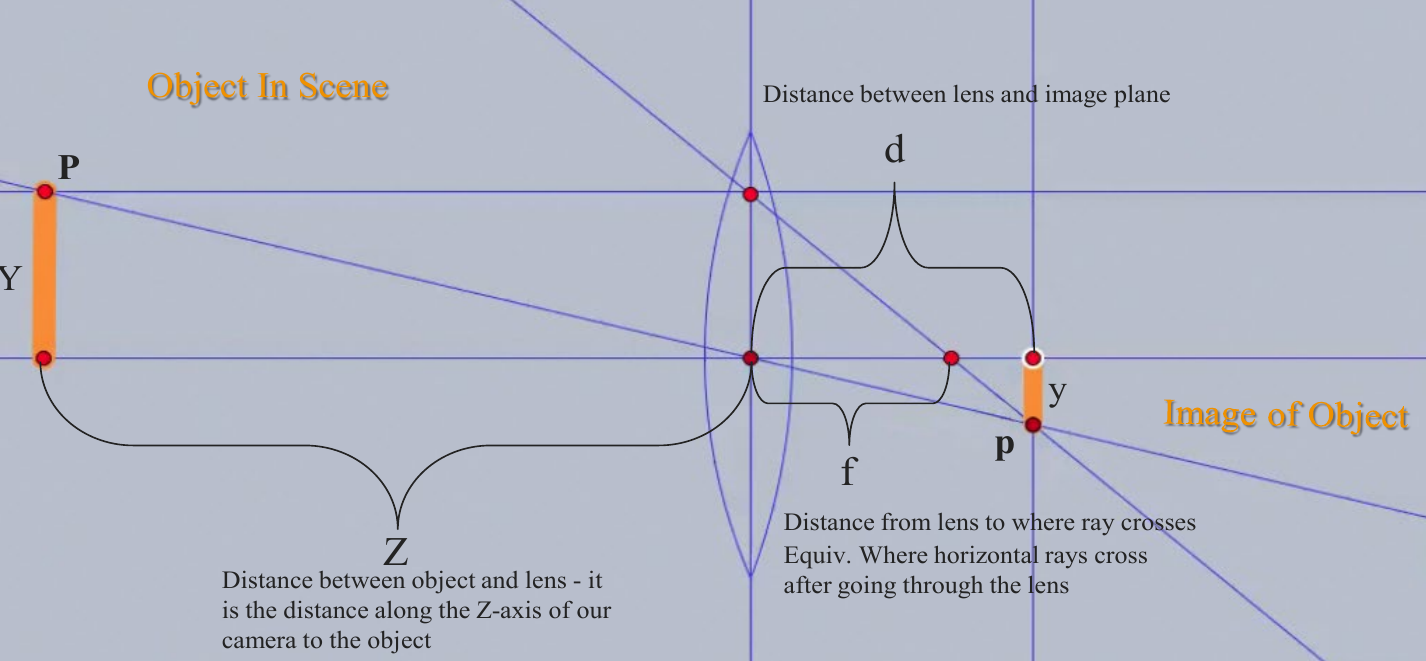
\includegraphics[width=\linewidth]{Images/Pinhole.png}
$1/f = 1/Z + 1/d$ \\
$Y/Z = y/d \Rightarrow y = d Y/Z$\\
Problem: d changes depending where the object is in the scene. Hence:
$y \approx f Y/Z$\\
\alert{Only valid if $Z >> d$}

\subsection*{Calibration}
\begin{itemize}
  \item Find $f$.
  \item Radial distortion:\\
    $r = norm(x, y), x' = x( 1 + k_1 t + k_2 r^2
    + k_3 r^3$\\
    (and similar for y)
\end{itemize}

\subsection*{Projection Equation}
$\begin{pmatrix} u\\ v\\ w\end{pmatrix} \sim
S \begin{pmatrix}r_1 & r_2 & r_3 & t \end{pmatrix}
\begin{pmatrix} X_w \\ Y_w \\ Z_w \\ 1\end{pmatrix}$ \\
$\begin{pmatrix} u\\ v\\ w\end{pmatrix} \sim
S \begin{pmatrix} ^C R_W & ^C T_W \end{pmatrix}
\begin{pmatrix} X_w \\ Y_w \\ Z_w \\ 1\end{pmatrix}$ \\
where $S = [f 0 x_0; 0 f y_0; 0 0 1]$\\
\includegraphics[width=\linewidth]{Images/projection.png}

\alert{$t$ is the distance from the camera to the world coordinate
system in camera coordinates}

\subsection*{Projective Geometry}
\begin{itemize}
  \item 
\end{itemize}

